
% Inbuilt themes in beamer
\documentclass[aspectratio=169]{beamer}
\usepackage{graphicx}
% Theme choice:
\usetheme{CambridgeUS}

% Title page details: 
\title{Econometrics Discussion Section 2: panel data} 
\author{John Green}
\date{Spring 2024}


\begin{document}

% Title page
\begin{frame}
    \titlepage 
\end{frame}

% Outline frame
\begin{frame}{Linearity assumption}
    \begin{itemize}
        \item We talk a lot about the OLS assumptions: conditional mean 0 of the error, finite 4th moments, no multicolinearity \dots
        \item Lurking under the hood: assumption the relationship is linear
        \item This is a very strong assumption: think about relationship between earnings and wages
        \item So we may try to relax the assumption of linearity and estimate a more flexible form; but we will focus on models which still fit into the framework of OLS
    \end{itemize}
\end{frame}

\begin{frame}{Polynomial function}
    \begin{itemize}
        \item If relationship between $Y$ and $X$ is not linear, we can try to approximate it by adding polynomials of $X$ into the regression: 
        \begin{itemize}
            \item $Y = \beta_0 + \beta_1 X + \beta_2 X^2 + \dots + \beta_3 X^n + u$
        \end{itemize}
        \item OLS works the same way! Just with new variables which are powers of $X$
        \item Difficult to interpret coefficients
        \item Question: How many factors should we had?
    \end{itemize}
\end{frame}

\begin{frame}{Log approximation}
    \begin{itemize}
        \item To a first approximation, $\log(1+x) \approx x$ for small $x$ (though be careful)
        \begin{itemize}
            \item This means we can think about a change in $\log(x)$ as a percentage change in $x$
        \end{itemize}
        \item Different ways to introduce logs into $Y=X\beta + u$. How should we interpret:
        \begin{itemize}
            \item log-linear
            \item linear-log
            \item log-log
        \end{itemize}
    \end{itemize}
\end{frame}

\begin{frame}{Log approximation}
    \begin{itemize}
        \item To a first approximation, $\log(1+x) \approx x$ for small $x$ (though be careful)
        \begin{itemize}
            \item This means we can think about a change in $\log(x)$ as a percentage change in $x$
        \end{itemize}
        \item Different ways to introduce logs into $Y=X\beta + u$. How should we interpret:
        \begin{itemize}
            \item \textbf{log-linear}: a change of $z$ in $X$ is associated with a $\beta z \%$ change in $Y$
            \item \textbf{linear-log}: a change of $z\%$ in $X$ is associated with a $\beta .0z \%$ change in $Y$
            \item \textbf{log-log}: a change of $z\%$ in $X$ is associated with a $\beta z \%$ change in $Y$
        \end{itemize}
        \item Other (actual) nonlinear forms are possible too
    \end{itemize}
\end{frame}

\begin{frame}{Non-linear least squares}
    \begin{itemize}
        \item These options (polynomials, logs) are still linear in the parameters
        \item But we can also estimate models which are nonlinear in the parameters using the non-linear least squares (NLLS) method
        \item Example:
        \begin{itemize}
            \item Logistic curve: $Y_i=\frac{1}{1+\exp \left(-\left(\beta_0+\beta_1 X_i\right)\right)}+u_i$
            \item Negative exponential: $Y_i=\beta_0\left[1-e^{-\beta_1\left(X_i-\beta_2\right)}\right]+u$
        \end{itemize}
        \item Still minimize the sum of squared residuals to find parameters, only now we need to use \textit{numerical methods} (eg gradient descent) rather than the closed form solution of OLS
    \end{itemize}
\end{frame}

\begin{frame}{Validity}
    \begin{itemize}
        \item \textit{Internal validity} means our study holds for the sample we have
        \item \textit{External validity} means we can generalize to the population
        \item External validity is hard, but even internal validity can fail:
        \begin{enumerate}
            \item OVB
            \item Wrong functional form (eg linear when we should have a polynomial)
            \item Errors-in-variables/measurement error
            \item Sample selection
            \item Simultaneous causality/endogeneity
        \end{enumerate}
        \item We have already talked about the first two; let's talk about the other three
    \end{itemize}
\end{frame}

\begin{frame}{Measurement error}
    \begin{itemize}
        \item Say the model is $Y_i = \beta_0 + \beta_1 X_i + u_i$
        \item But instead of observing $X_i$, we observe $X_i^* = X_i + v_i$, ie a noisy signal
        \item Then we estimate 
        $$Y_i = \beta_0 +  \beta_1 X_i^* + u_i = \beta0 + \beta_1 (X_i + v_i) + u_i $$
        $$ \to \beta0 + \beta_1 X_i + (\beta_1 v_i + u_i)  = \beta0 + \beta_1 X_i + u_i^*$$
        \item This introduces measurement error bias: $\hat{\beta}_1 \rightarrow_p \beta_1 \frac{\sigma_X^2}{\sigma_X^2+\sigma_V^2}$
        \item Notice direction of bias is constant!
    \end{itemize}
\end{frame}

\begin{frame}{Sample selection}
    \begin{itemize}
        \item If data are missing non-randomly due to the value of the dependent variable, we have a problem
        \item Example: we only observe wages for people who are employed
        \begin{itemize}
            \item \href{notebook}{https://tinyurl.com/polyecon}
        \end{itemize}
        \item Solutions:
        \begin{itemize}
            \item Filter your sample
            \item RCT
            \item Model the selection bias
        \end{itemize}
    \end{itemize}
\end{frame}

\begin{frame}{Simultaneous Causality}
    \begin{itemize}
        \item Most of the time, $X \to Y$ \textit{and} $Y \to X$; think about supply and demand 
        \item This will introduce endogeneity into our model
        \item So, we need to somehow control for the endogeneity; can use an instrumental variable (IV) or an RCT (which is really a type of IV)
    \end{itemize}
\end{frame}

\begin{frame}{Panel data}
    \begin{itemize}
        \item Panel data has many advantages; in particular it let's us control for OVB so long as the omitted variable is constant over time
        \item We can \textit{demean} the data: subtract the mean of each variable from each observation
        \item We can \textit{difference} the data: subtract the previous observation from each observation (only if $T-2$)
        \item We can add in $N-1$ dummy variables, to control for each unit
        \item But we need to be careful! If we have measurement error, differencing will amplify it
    \end{itemize}
\end{frame}

\begin{frame}{First differences}
    \begin{itemize}
        \item Suppose we have two periods of data: $\{X_{it},Y_{it} \}_{i<=N, t<=2}$
        \item Our model is $Y_{it} = \beta_0 + \beta_1 X_{it} + \alpha_i + u_{it}$
        \item So take 
        $$Y_{i1} - Y_{i2} = \beta_0 + \beta_1 X_{i1} + \alpha_i + u_{i1} - \beta_0 - \beta_1 X_{i2} - \alpha_i - u_{i2}$$
        $$ = \beta_1 (X_{i1}-X_{i2}) - \tilde{u_i}$$
        \item So we regress change in $Y$ on change in $X$ and get a consistent estimate of $\beta_1$
    \end{itemize}
\end{frame}

\begin{frame}{Time fixed effects}
    \begin{itemize}
        \item Some things might vary across time, but not across units (national interest rate)
        \item We can de-mean based on \textit{time} rather than unit
        \item Include $T-1$ binary dummy variables 
        \item Or, take the difference (if $T=2$); then we include a slope in the difference equation
    \end{itemize}
\end{frame}

\begin{frame}{Assumptions for panel least squares}
    \begin{itemize}
        \item 3 and 4 still the same: finite 44\textsuperscript{th} moment (outliers are rare) and no multicolinearity
        \item Conditional mean is different, need to condition on all periods of unit $i$ plus the fixed effect: $E\left(u_{i t} \mid X_{i 1}, \ldots, X_{i T}, \alpha_i\right)=0$
        \item $\left(X_{i 1}, \ldots, X_{i T}, u_{i 1}, \ldots, u_{i T}\right), i=1, \ldots, n$ are i.i.d. across $i$
        \item Also need to watch out for \textit{autocorrelation}, when $corr(u_{i,t},u_{i,t+s}) \neq 0$ for some $s$
        \begin{itemize}
            \item This will often be the case!
            \item If we ignore, our standard errors will be too small; just like for heteroskedasticity
            \item So, \textit{cluster} standard errors by unit
        \end{itemize}
    \end{itemize}
\end{frame}

\begin{frame}{Linear probability model}
    \begin{itemize}
        \item Say we have some outcome $D \in \{0,1\}$ and some regressor $X$
        \item We might try to model $D_i = \beta_0 + \beta_1 X_i + u_i$, where $\hat{D_i}$ is the probability that $D_i = 1$
        \item Good: $\beta$ is easy to interpret
        \item Also good: inference is straightforward, $R^2$ works normally, etc.
        \item Bad: $\hat{D_i}$ can be $< 0$ or $> 1$, which does not make sense
        \item Also bad: change in probability is linear (can we relax this?)
    \end{itemize}
\end{frame}


\begin{frame}{Non-linear probability model}
    \begin{itemize}
        \item Probit: $Pr \left(Y=1 \mid X_1, X_2\right)=\Phi\left(\beta_0+\beta_1 X_1+\beta_2 X_2\right)$
        \begin{itemize}
            \item $ z = \beta_0+\beta_1 X_1+\beta_2 X_2 $ is the z-score, so a change in $X_1$ shifts the z-score by $\beta_1$
        \end{itemize}
        \item logit: $Pr (Y=1 \mid X) = \frac{1}{1+e^{-\left(\beta_0+\beta_1 X\right)}}$
        \item Both valid choices, doesn't really matter which you use
        \item Estimate numerically, just like for the non-linear least squares:
    solve $ \min _{b_0, b_1} \sum_{i=1}^n\left[Y_i-\Phi\left(b_0+b_1 X_i\right)\right]^2$
    \end{itemize}
\end{frame}

\begin{frame}{Maximum Likelihood Estimation (MLE)}
    \begin{itemize}
        \item In practice, we use the \textit{maximum-likelihood estimator}: instead of \textit{minimizing} a sum of squared errors, we will choose parameters to \textit{maximize} the ``likelihood function``
        \item This estimate will be consistent, efficient, and normally distributed 
        \item The specific form of the likelihood function depends on the problem you are solving, but intuition is familiar
        \begin{itemize}
            \item With a t-test, we knew the distribution under $H_0$ and asked: given this distribution, how likely was it we would observe our data?
            \item MLE turns that around, and asks: given our data, what is the most likely distribution that it comes from?
            \item Find the parameters for that distribution
        \end{itemize}
        \item We can evaluate the fit from a logit or a probit using the fraction correctly predicted or a psueudo-$R^2$
    \end{itemize}
\end{frame}

% \begin{frame}
%     \centering
%     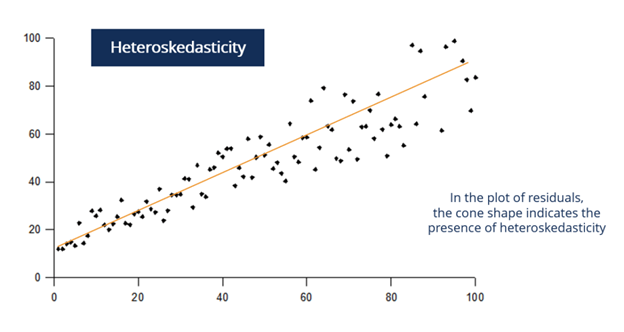
\includegraphics[width = .75\textwidth,keepaspectratio]{./figs/heteroskedasticity.png}
% \end{frame}


\end{document}